\begin{figure*}[t!]
  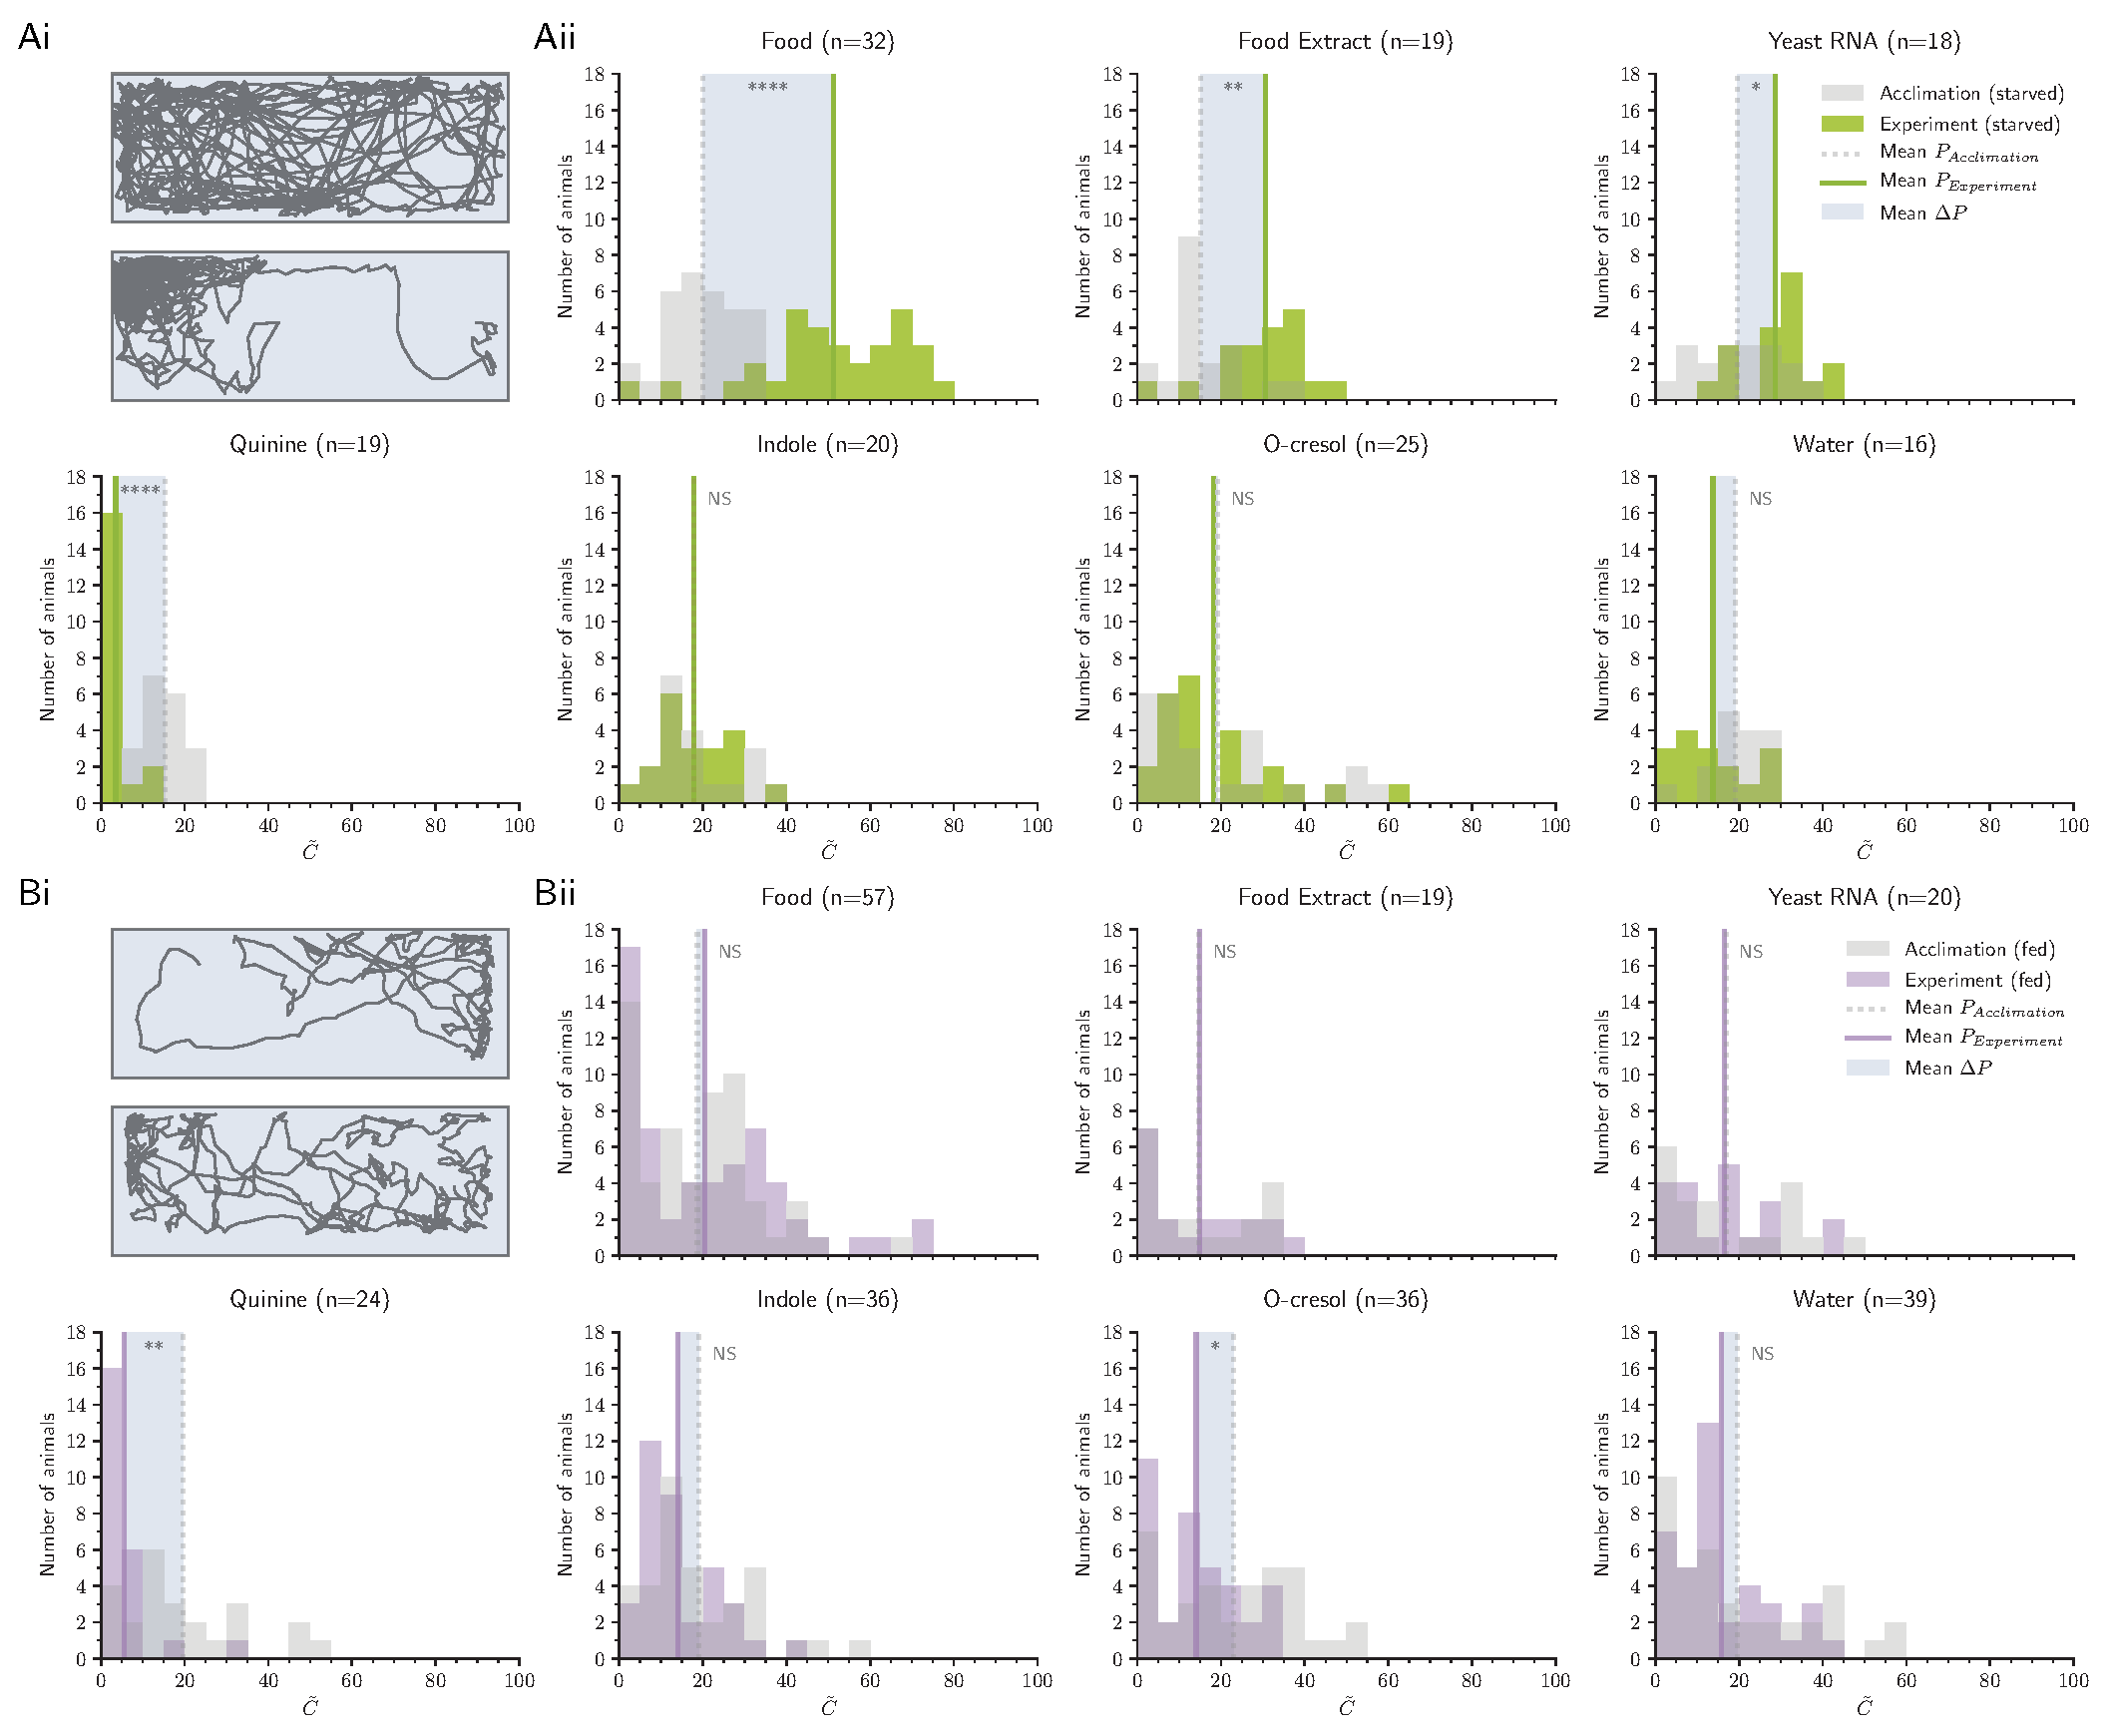
\includegraphics[width=\textwidth]{Figures/images/2.eps}
  \caption{\textbf{ Physiological feeding state affects larval attraction towards ecologically relevant odors.} Ai: Example trajectory of a starved larva during the acclimation (top) and the experiment phase (below), responding to food stimulus. Aii: Distribution of larvae during the acclimation phase (grey) and experiment phase (green), mean concentration ${\tilde{C}}$. The shaded box visualizes the mean ${\Delta}$P. Note that due to the unequal distribution of high and low concentration areas in the behavior arena, animals naturally appear to distribute near lower concentrations when no stimulus is present. Bi: Example trajectory of a fed larva during the acclimation (top) and experiment phase (below), responding to food stimulus. Bii: Distribution of fed larval preference during the acclimation (grey) and experiment phase (purple). In Aii and Bii, asterisks denote the significance level of paired-sample Welch's t-tests comparing acclimation P and experiment P (NS: not significant). N values reported next to each stimulus describe the number of animals in the treatment.
 }
\end{figure*}